\documentclass[10pt,a4paper]{article}

%% PACKAGES WITH OPTIONS
\usepackage[english]{babel}
\usepackage[T1]{fontenc}
\usepackage[utf8]{inputenc}
\usepackage[version=4]{mhchem} % Chemistry and isotopes with \ce{} (other option: 'chemformula' \ch{})
\usepackage[numbers]{natbib} % numbers: needed argument, otherwise error
\usepackage[section]{placeins} % Place floats in their own section
\usepackage[nottoc,notlot,notlof]{tocbibind} % Include bibliography in table of contents

%% PACKAGES WITHOUT OPTIONS
\usepackage{amsmath, amsfonts, amssymb}
\usepackage{enumitem} % Lists
\usepackage{flafter} % Place floats after their first appearance in text
\usepackage{float} % [H] modifier for floats etc.
\usepackage{graphicx}
\usepackage{hyperref, cleveref} % Creates links (boxes in various colors around words)
\usepackage{indentfirst} % Always indent the first line of a section
\usepackage{listings} % Typesetting source code
\usepackage{physics} % Vector calculus etc.
\usepackage{siunitx} % Fancy display of SI units
\usepackage{subcaption} % Enables subfigures
\usepackage{titling}
\usepackage{xcolor} % Anything with color e.g. \fcolorbox{black}{red}{}
\usepackage{xurl} % Loads package 'url' and breaks urls nicely

%% PACKAGES SETUP COMMANDS
\hypersetup{colorlinks=true,urlcolor=blue}

%% COMMANDS
% Bold and italic vector symbols (preferably use \vb{} instead)
\renewcommand{\vec}[1]{\boldsymbol{#1}}
% Monospaced inline code (for multiline code, use package 'listings')
\newcommand{\code}[1]{\texttt{#1}}
% Equals sign, with number above referencing some equation
\newcommand{\numeq}[1]{\stackrel{\scriptscriptstyle(\mkern-1.5mu#1\mkern-1.5mu)}{=}}
% If-and-only-if sign, with number above referencing some equation
\newcommand{\numiff}[1]{\stackrel{\scriptscriptstyle(\mkern-1.5mu#1\mkern-1.5mu)}{\Leftrightarrow}}
% Numbers a single line in a no-numbering multiline equation* or align*
\newcommand{\numberthis}{\addtocounter{equation}{1}\tag{\theequation}}

%% TITLE VARIABLES
\author{Jonathan Maes}
\title{Biaxial nanomagnets as building block for balanced half-adders}


\begin{document}
	\begin{titlingpage}
	\maketitle
	\end{titlingpage}

	\pagenumbering{roman}
	\newpage
	
	\tableofcontents
	\pagenumbering{arabic}
	\newpage

	\section{Introduction}
	% === \usepackage TESTS ===
	% === This comment's only purpose is a git sync test. ===
	Probably MuMax3 will be used.~\cite{MuMax3}
	An interesting source is~\cite{NML_Carlton}.
	Also a good introduction to the main equations is found in \cite{MuMax3_advances}.
	
	\section{Physics}
	% === THE FOLLOWING IS A NONCOMPREHENSIVE SUMMARY OF THE PHYSICS ===
	\subsection{Landau-Lifschitz-Gilbert equation}
	\begin{equation}
		\frac{\partial m}{\partial t} = - \gamma_0 \vb{m} \cross \vb{H_{eff}} - \lambda \vb{m} \cross (\vb{m} \cross \vb{H_{eff}})
	\end{equation}
	PDE requires an effective field $\vb{H_{eff}}$ which is defined as
	\begin{equation}
		\vb{H_{eff}} = - \frac{1}{\mu_0} \frac{\partial E}{\partial \vb{M}}
	\end{equation}
	the energy $E$ is the sum of several contributions, all explained in the next section.
	
	\subsection{Energy contributions}
	\subsubsection{Exchange energy}
	Tries to align neighboring spins:
	$E_{i,j} = -J \vb{S_i} \vdot \vb{S_j}$
	\subsubsection{Magnetostatic energy/Demagnetization energy}
	I think:
	\begin{align}
		\div{\vb{B}} &= 0 \\
		\vb{B} &= \mu_0 (\vb{H} + \vb{M})
	\end{align}
	means that a given $\vb{M}$ must result in a certain $\vb{H}$, which is then called $\vb{H}_{demag}$.
	($\vb{H}$ is gradient of scalar field $u$)
	
	\subsubsection{Anisotropy energy}
	Only even orders in Taylor expansion are considered, in order to fulfill $E(\vb{m}_{min}) = E(-\vb{m}_{min})$. Then $K_{u1}, K_{u2}, \dots$ for order 2, 4, ... respectively.
	
	There is uniaxial, and there is cubic, and there is many other options which are rarely used.
	
	\subsubsection{Zeeman energy}
	Energy of magnetization in an external field.
	$E = -\mu_0 \vb{M} \cdot \vb{H_{ext}}$
	
	\section{Tests}
	\subsection{Random thermal switching}
	\subsubsection{Preparation}
	Step 1: find energy barrier \\
	The procedure used is to set both $m$ and $B_{ext}$ at an angle ($\abs{B_{ext}} = \SI{5}{\tesla}$) and then \code{minimize()}.
	
	Step 2: random switching over \SI{100}{\nano\second} \\
	In GYP-18~\cite{GYP-18} the formula
	\begin{equation}
	    t_i = -\frac{1}{f_0} \exp(\frac{\Delta E_i}{k_B T}) \ln(1-P_i)
	\end{equation}
	appears, with $f_0 = \SI{e12}{\hertz}$ attempt frequency, and $P_i$ random between 0 and 1. The average value of $-\ln(1-P_i)$ is then $\ln(4) \approx 1.4$ (?). To get an average $t_i = \SI{100}{\nano\second}$ at $T=\SI{300}{\kelvin}$, one should therefore have
	\begin{equation}
	    \Delta E_i = k_B T \ln(\frac{f_0 t_i}{\ln(4)}) = 11.186 k_B T = \SI{0.289}{\electronvolt} \mathrm{.}
	\end{equation}
	This seems pretty high tbh
	Also there is another formula in mumax3~\cite{MuMax3}
	
	Observation: with a barrier height approximately equal to $k_B T$, a switching speed of about \SI{100}{\nano\second} is observed.
	
	Question: should $\alpha$ be 0.1 always, i guess this is just a case of ``0.1 works so we use 0.1''
	
	\subsubsection{Results}
	Step 1: find energy barrier \\
	With perfectly circular geometry (i.e. \\
	\code{geometry := Ellipse(100e-9, 100e-9)} \\
	\code{geometry = geometry.Add(Ellipse(100e-9, 100e-9).RotZ(Pi/2))}) \\
	there is still shape anisotropy, but with opposite sign (what are maxima in actual plus-figures are now minima)
	
	Findings (for \SI{100}{\nano\metre} long axis ellipse plus-sign):
	at \SI{45}{\nano\metre} the preferred directions switch from the axes (\SI{0}{\degree}) to in between the axes (\SI{45}{\degree}),
	at \SI{65}{\nano\metre} the anisotropy with preferred \SI{0}{\degree} direction is the strongest
	
	After running for \SI{1}{\micro\second} at \SI{300}{\kelvin}, with shape \SI{65}{\nano\metre} by \SI{100}{\nano\metre} ellipses in plus shape, the following angles were observed (\cref{fig:biaxial_island:1microsecond_300K}):
	\begin{figure}
	    \centering
	    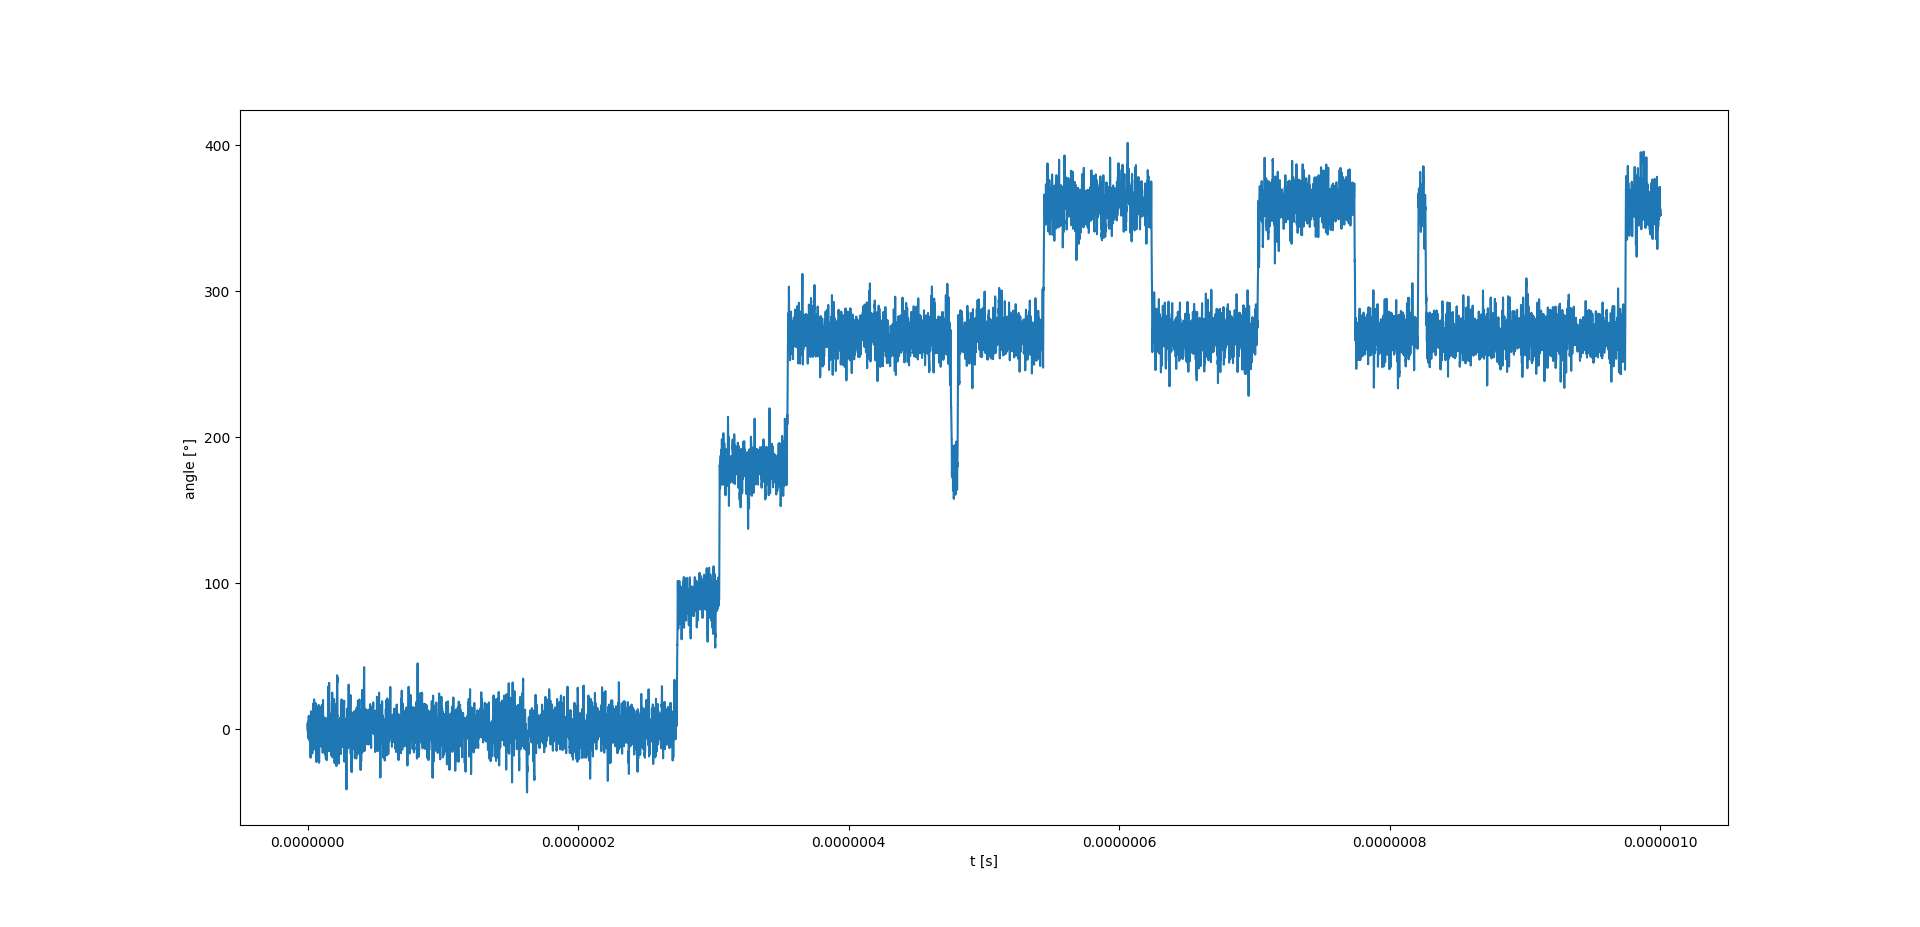
\includegraphics[width=1.0\columnwidth]{Figures/biaxial_island/table.png}
	    \caption{\SI{1}{\micro\second} at \SI{300}{\kelvin}}
	    \label{fig:biaxial_island:1microsecond_300K}
	\end{figure}
	
	
	\newpage
	\bibliographystyle{IEEEtran}
	\bibliography{bibliography/bibliography.bib}
\end{document}
